\documentclass[12pt, a4paper]{report}

% ==============================================================================
% 1. PACKAGES FONDAMENTAUX & GESTION LINGUISTIQUE
% ==============================================================================
\usepackage[utf8]{inputenc}       % Encodage des caractères sources (UTF-8)
\usepackage[T1]{fontenc}          % Encodage de sortie 8 bits pour césures françaises
\usepackage[french]{babel}        % Typographie, césures et ponctuation françaises
\usepackage{lmodern}              % Police vectorielle standard Latin Modern
\usepackage{microtype}            % Amélioration micro-typographique (justification optique)

% ==============================================================================
% 2. GÉOMÉTRIE DE PAGE & INTERLIGNE ACADÉMIQUE
% ==============================================================================
% Marges conformes aux standards universitaires (3 cm gauche pour reliure, 2.5 cm autres)
\usepackage[
    a4paper,
    left=3cm,
    right=2.5cm,
    top=2.5cm,
    bottom=2.5cm
]{geometry}

\usepackage{setspace}
\onehalfspacing                   % Interligne 1,5 académique

% Espacement vertical des paragraphes et alinéa
\setlength{\parskip}{0.5em}
\setlength{\parindent}{1.5em}

% ==============================================================================
% 3. PACKAGES TABLEAUX & COULEURS
% ==============================================================================
\usepackage{tabularx}             % Tableaux à largeur automatique (colonnes X ajustables)
\usepackage{array}                % Personnalisation avancée des colonnes
\usepackage{booktabs}             % Filets professionnels (toprule, midrule, bottomrule)
\usepackage[table]{xcolor}        % Gestion des couleurs et ombrages de lignes de tableaux

% ==============================================================================
% 4. GESTION DES FIGURES & ROTATION DE PAGE (PAYSAGE)
% ==============================================================================
\usepackage{graphicx}             % Inclusion d'images (PDF, PNG, JPEG)
\usepackage{pdflscape}            % Pages en mode Paysage visibles directement en PDF
\usepackage{caption}              % Personnalisation des légendes
\captionsetup{
    font=small,
    labelfont=bf,
    labelsep=colon,
    justification=centering
}

% ==============================================================================
% 5. LIENS HYPERTEXTES ET RÉFÉRENCES CROISÉES
% ==============================================================================
\usepackage{hyperref}
\hypersetup{
    colorlinks=true,
    linkcolor=black,              % Liens internes en noir pour impression académique
    citecolor=black,
    urlcolor=blue,
    pdftitle={Chapitre 3 : Conception et mise en oeuvre de la solution Zalisk},
    pdfauthor={Mémoire de Licence}
}

% ==============================================================================
% DÉBUT DU DOCUMENT
% ==============================================================================
\begin{document}

% Initialisation du compteur pour débuter directement au Chapitre 3
\setcounter{chapter}{2}

\chapter{Conception et mise en œuvre de la solution Zalisk}
\label{chap:conception-mise-en-oeuvre}

% ------------------------------------------------------------------------------
% 3.1 INTRODUCTION
% ------------------------------------------------------------------------------
\section{Introduction}
\label{sec:introduction}

À la suite de la présentation des solutions existantes, de l'analyse des besoins et de la proposition de la solution Zalisk, ce chapitre est consacré à sa conception et à sa mise en œuvre. Zalisk est une plateforme SaaS destinée à faciliter la gestion des demandes de service après-vente (SAV) au sein des entreprises.

Ce chapitre présente dans un premier temps la conception générale de la solution, sa modélisation et son architecture technique. Il aborde ensuite la mise en œuvre de ses principales fonctionnalités, avant de présenter les choix techniques effectués, les mécanismes de sécurité adoptés et les difficultés rencontrées. Enfin, les principales interfaces réalisées seront présentées, accompagnées d'une vérification des fonctionnalités et d'une analyse des résultats obtenus ainsi que des limites de la solution.

% ------------------------------------------------------------------------------
% 3.2 CONCEPTION GÉNÉRALE DE LA SOLUTION
% ------------------------------------------------------------------------------
\section{Conception générale de la solution}
\label{sec:conception-generale}

% ------------------------------------------------------------------------------
% 3.2.1 APPROCHE DE CONCEPTION
% ------------------------------------------------------------------------------
\subsection{Approche de conception}
\label{subsec:approche-conception}

La conception de Zalisk repose sur une démarche progressive visant à traduire les besoins fonctionnels et techniques identifiés au chapitre précédent en une organisation cohérente du système. Cette démarche consiste à définir les fonctionnalités attendues, les interactions entre les différents acteurs, la structure des données ainsi que les mécanismes nécessaires au fonctionnement de la plateforme.

Pour décrire et structurer le système, nous nous appuyons sur le langage de modélisation UML. Celui-ci permet de représenter les différents aspects de la solution, notamment les fonctionnalités accessibles aux acteurs, l'organisation des données, le déroulement des processus et les interactions entre les composants. Ces représentations facilitent la compréhension du système et servent de support à sa conception.

La conception tient également compte des caractéristiques propres à Zalisk. Son fonctionnement multi-entreprise doit permettre à plusieurs entreprises de partager un même environnement applicatif tout en préservant la séparation de leurs données et de leurs espaces de travail. Elle prend aussi en considération la complémentarité entre les agents humains, chargés du traitement des demandes SAV, et l'assistance par intelligence artificielle, qui intervient pour apporter des réponses automatisées et faciliter le transfert vers un agent lorsque cela est nécessaire.

% ------------------------------------------------------------------------------
% 3.2.2 ARCHITECTURE FONCTIONNELLE ET IDENTIFICATION DES ACTEURS
% ------------------------------------------------------------------------------
\subsection{Architecture fonctionnelle et identification des acteurs}
\label{subsec:architecture-fonctionnelle-acteurs}

L'architecture fonctionnelle de Zalisk s'organise autour de deux espaces principaux : le portail public, destiné aux clients, et le Workspace Entreprise, réservé aux équipes des entreprises. Ces espaces regroupent les fonctionnalités nécessaires à la gestion et au traitement des demandes de service après-vente.

Le portail public permet aux clients de rechercher une entreprise dans l'annuaire, de consulter les informations relatives à ses agences et de soumettre une demande d'assistance sans créer de compte. Le Workspace Entreprise met à disposition des équipes les outils de gestion des tickets, des conversations, des compétences, des succursales et des abonnements.

La plateforme fait intervenir cinq principaux acteurs, présentés dans le tableau suivant :

\begin{table}[htbp]
    \centering
    \caption{Identification des acteurs de Zalisk et leurs responsabilités}
    \label{tab:acteurs-zalisk}
    \renewcommand{\arraystretch}{1.35}
    \begin{tabularx}{\textwidth}{|>{\bfseries}p{4.2cm}|X|}
        \hline
        \rowcolor[gray]{0.92} Acteur & Rôle et responsabilités \\
        \hline
        Client & Accède au portail public, dépose des réclamations et échange directement avec le service SAV. \\
        \hline
        Conseiller SAV & Prend en charge les tickets, suit les délais de traitement (SLA, \textit{Service Level Agreement}), dialogue avec les clients et rédige des notes internes. \\
        \hline
        Superviseur SAV & Supervise les files d'attente, réaffecte les tickets, gère les compétences des agents et coordonne les succursales. \\
        \hline
        Administrateur de l'entreprise & Invite les membres, attribue les rôles, gère les abonnements et paramètre les fonctionnalités de l'espace de travail. \\
        \hline
        Propriétaire de l'espace & Détient les droits de propriété sur l'espace de l'entreprise et dispose des privilèges les plus élevés, notamment concernant sa suppression. \\
        \hline
    \end{tabularx}
\end{table}

L'architecture fonctionnelle prévoit également un module d'assistance par intelligence artificielle reposant sur le mécanisme RAG. Celui-ci permet d'exploiter les documents de référence afin de générer des propositions de réponses et de transférer les demandes vers un agent humain lorsque cela est nécessaire. Ce module constitue une composante cible de la plateforme.

La figure suivante présente l'organisation fonctionnelle de Zalisk, les cinq acteurs de la plateforme, leurs espaces d'accès respectifs ainsi que les principaux modules et les relations fonctionnelles entre ces différents éléments.

% ==============================================================================
% INSERTION DU DIAGRAMME D'ARCHITECTURE FONCTIONNELLE
% ==============================================================================
% Note d'intégration pour pdfLaTeX :
% Le fichier vectoriel "figures/architecture-fonctionnelle.pdf" (généré à partir du SVG)
% est inclus directement sans nécessiter l'option --shell-escape.
% Comme le diagramme est au format paysage (ratio 2:1), il est disposé sur une page
% dédiée en orientation Paysage via l'environnement {landscape} pour une lisibilité optimale.
% ==============================================================================

\begin{landscape}
\begin{figure}[p]
    \centering
    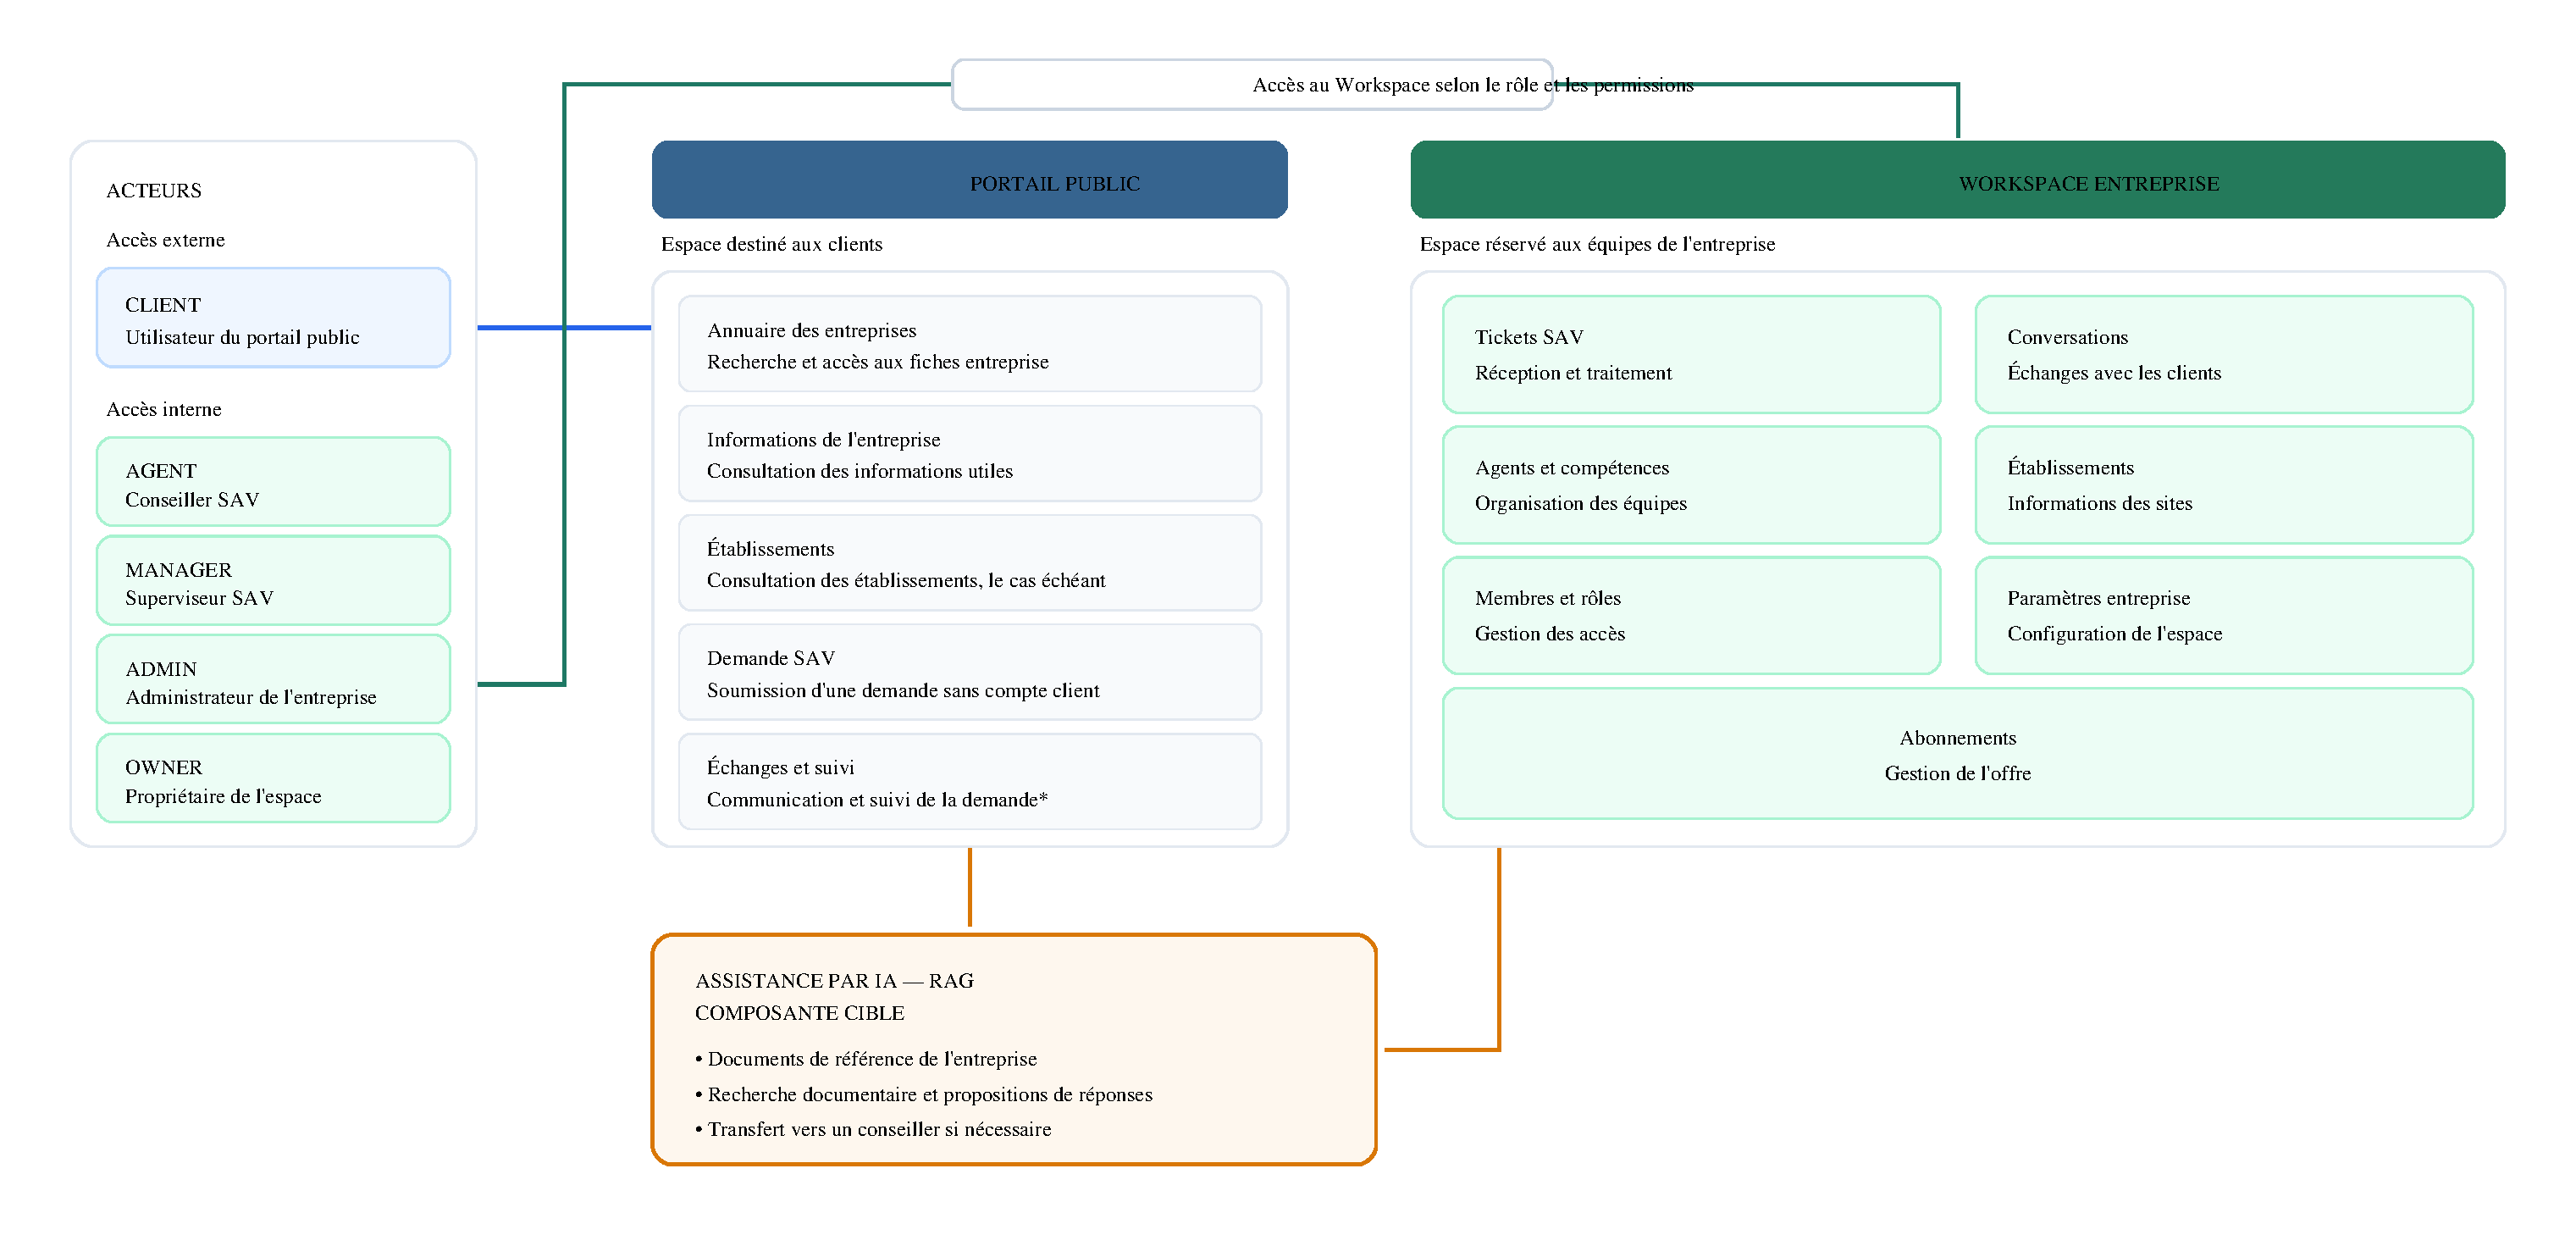
\includegraphics[width=0.96\linewidth]{figures/architecture-fonctionnelle.pdf}
    \caption{Architecture fonctionnelle de Zalisk}
    \label{fig:architecture-fonctionnelle}
\end{figure}
\end{landscape}

% ------------------------------------------------------------------------------
% VARIANTE ALTERNATIVE EN MODE PORTRAIT :
% Si vous préférez intégrer la figure directement sur une page portrait sans rotation,
% décommentez le bloc ci-dessous et commentez le bloc {landscape} ci-dessus :
%
% \begin{figure}[htbp]
%     \centering
%     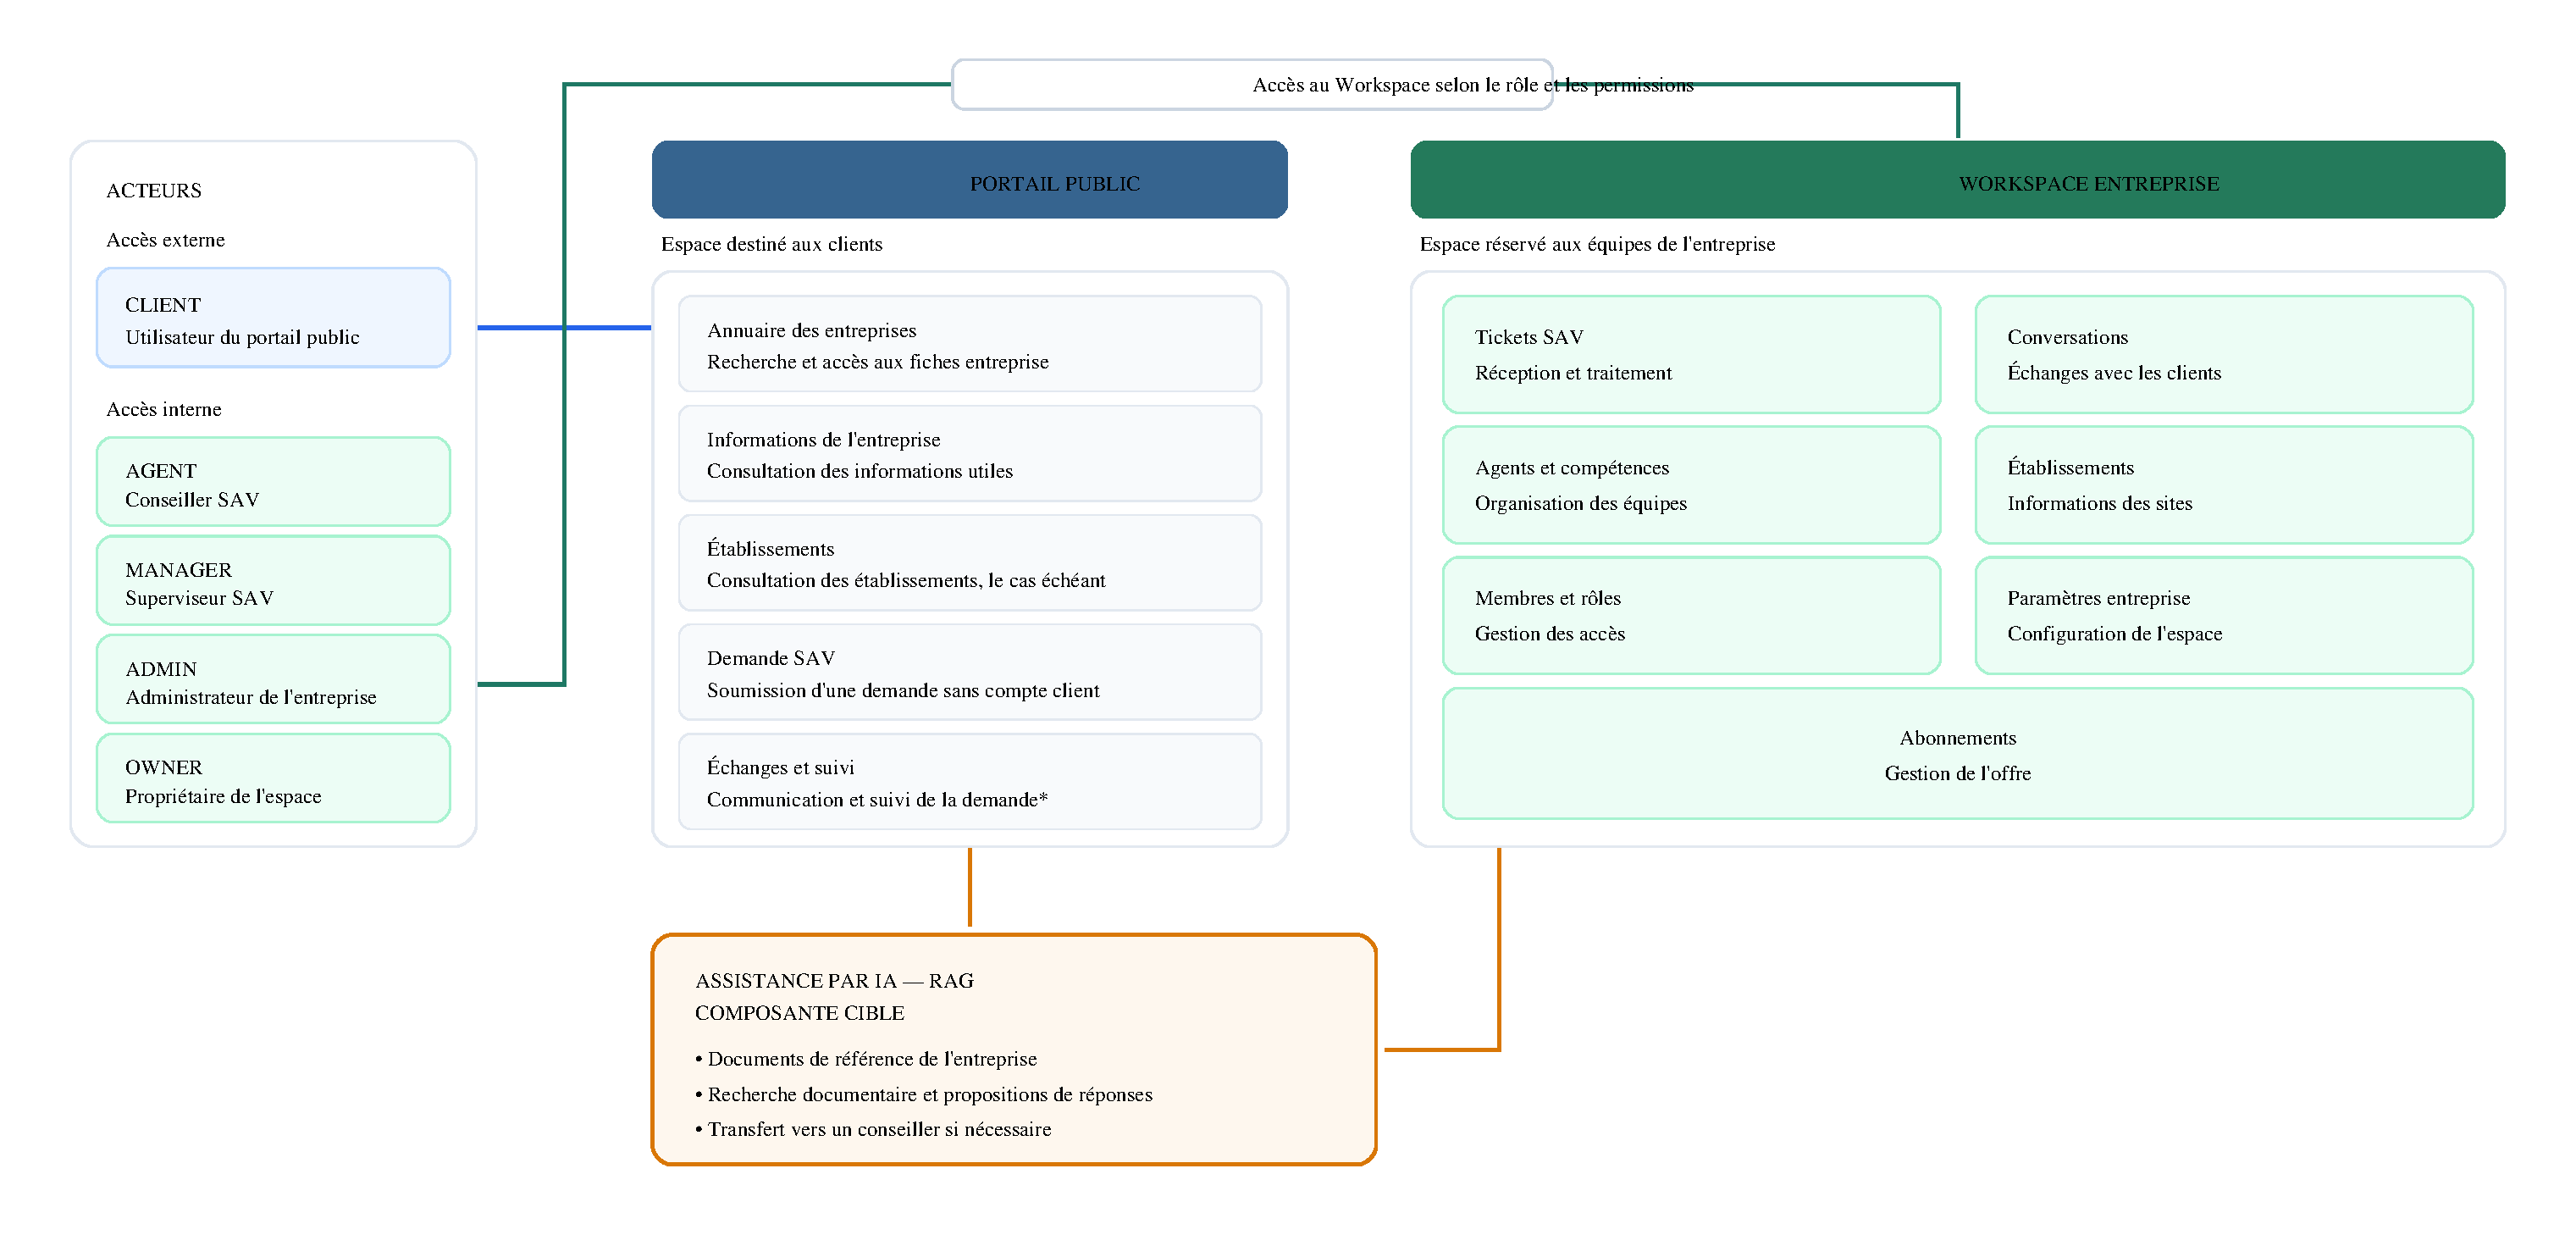
\includegraphics[width=\textwidth]{figures/architecture-fonctionnelle.pdf}
%     \caption{Architecture fonctionnelle de Zalisk}
%     \label{fig:architecture-fonctionnelle}
% \end{figure}
% ------------------------------------------------------------------------------

% ------------------------------------------------------------------------------
% 3.2.3 DESCRIPTION DES PROCESSUS DE TRAITEMENT DES DEMANDES SAV
% ------------------------------------------------------------------------------
\subsection{Description des processus de traitement des demandes SAV}
\label{subsec:processus-traitement-sav}

Le traitement des demandes de service après-vente dans Zalisk repose sur un processus permettant d'assurer la réception, la prise en charge et le suivi des sollicitations des clients. Il met en relation le portail public, utilisé par les clients pour contacter une entreprise, et le Workspace Entreprise, dans lequel les équipes SAV assurent le traitement des demandes.

Le processus commence lorsqu'un client accède au portail public d'une entreprise et soumet une demande d'assistance. Celle-ci est enregistrée dans la plateforme sous la forme d'un ticket, qui constitue le support de suivi de la réclamation. Le client peut ensuite échanger avec le service SAV afin de fournir des informations complémentaires ou d'obtenir des précisions sur l'évolution de sa demande.

Du côté de l'entreprise, les conseillers SAV accèdent aux tickets depuis leur espace de travail. Ils analysent les demandes, communiquent avec les clients et effectuent les actions nécessaires à leur résolution. Le superviseur SAV intervient dans la coordination de cette activité, notamment lorsque la répartition ou la réaffectation des tickets nécessite une intervention. Les échanges et les actions réalisés au cours du traitement permettent de conserver un historique des interventions.

La plateforme prévoit également un module d'assistance par intelligence artificielle fondé sur l'approche RAG. Dans son fonctionnement cible, ce module exploite les documents de référence de l'entreprise afin de proposer des réponses aux demandes des clients. Lorsque la réponse générée ne permet pas de résoudre la demande ou qu'une intervention humaine est nécessaire, la conversation peut être transférée à un conseiller SAV afin d'assurer la continuité du traitement.

\end{document}
